\subsection{Assemblage}
La connection du capteur AD8232 avec la carte ESP32 doit suivre le schéma suivant :

\begin{figure}[H]
  \centering
  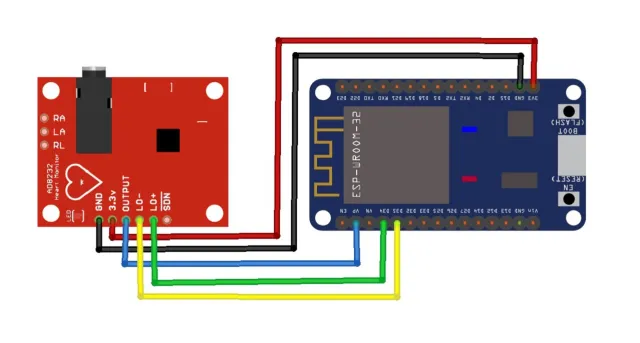
\includegraphics[scale=.4]{imgs/AD8232ESP32.png}
  \caption{Interfaçage du capteur AD8232 avec la carte de développement ESP32}
\end{figure}

Pour que le système soit en marche, il faut ajouter :
\begin{enumerate}
  \item une connexion INTERNET : la carte ESP32 peut se connecter à un réseau WIFI. Mais un tel réseau doit assurer une connexion à INTERNET et n'est pas un simple réseau local par exemple.
  \item un serveur de données : il faut avoir un accès à un serveur dans le WEB afin d'y enregistrer les informations récupérées du capteur. Ainsi, une inscription dans une plateforme dédiée peut donner ce type d'accès.
\end{enumerate}

Jusqu'à présent, la partie hardware du projet a été investiguée. En se basant sur cette architecture, quels sont les composants software à ajouter permettant le bon fonctionnement du système ?